\chapter{Nuova Fisica a CMS}
\label{cap:TerzoCapitolo}
\let\cleardoublepage\clearpage

Proposto inizialmente nel 1961 da Sheldon Glashow, e raffinato da Steven Weinberg e Abdus Salam nel 1968, il Modello Standard (SM) rappresenta ad oggi una delle teorie più consolidate nella fisica moderna. Esso descrive le tre interazioni che agiscono tra le particelle fondamentali che costituiscono la materia: l'interazione Forte, responsabile del legame tra nucleoni nei nuclei atomici, l'interazione Debole, responsabile di processi come decadimento $\beta$ e l'interazione Elettromagnetica che governa le forze tra particelle cariche. La Gravità, pur essendo una forze fondamentale, non rientra nella struttura del Modello Standard. \newline
Il beneficio di avere un frame completo come il Modello Standard risiede nella capacità di prevedere il comportamento di particelle subatomiche conoscendo la struttura teorica alla base: in questo contesto una delle maggiori conquiste dello SM è la scoperta del bosone di Higgs, teorizzato per la prima volta da Higgs nel 1964 e rilevato a CMS nel 2012.

Nel Modello Standard esistono particelle instabili che possono essere considerate \textit{Long Lived} (LLPs) a causa della loro vita media relativamente elevata rispetto alle scale temporali tipiche di processi subatomici. Al Large Hadron Collider, LLPs possono essere prodotte dalla collisione protone protone, venendo rilevate nei detector nel momento del decadimento: ciò infatti porta alla produzione di tracce di particelle visibili che non sono state originate nel punto di interazione nominale della collisione.\newline
Dato un numero iniziale di particelle prodotte $N_0$ e il tempo di decadimento proprio delle stesse $\tau$, ovvero il tempo di decadimento calcolato nel sistema di riferimento a riposo della particella, il numero di particelle restanti dopo un tempo $t$ segue la legge esponenziale nel sistema di riferimento a riposo: 

\begin{equation}
  \label{eq:ExponentialDecay}
  N(t) = N_0 e^{-t/\tau}
\end{equation}

Lo spostamento $L$ corrispondente al tempo di decadimento $\tau$ nel sistema del laboratorio è moltiplicato dal fattore di Lorentz $\gamma = 1/\sqrt{1-\beta^2}$, essendo i prodotti di decadimento ad una velocità comparabile alla velocità della luce $c$:

\begin{equation}
  \label{eq:LorentzBoost}
  L = \gamma \beta c \tau
\end{equation}


Affinché una particella abbia un tempo di vita medio elevato il decadimento deve essere soppresso e questo può avvenire secondo due meccanismi differenti \cite{Genest:2022}: un accoppiamento debole dei mediatori di decadimento, oppure da uno spazio delle fasi ristretto. \newline
Questi meccanismi giocano un ruolo importante nel Modello Standard: in esso infatti sono presenti LLPs come pioni carichi ($\tau_{\pi^\pm} = 26\si{ns}$), muoni ($\tau_{\mu} = 2.2 \si{\mu s}$) e neutroni ($\tau_{n} = 880\si{s}$).

\section{Ricerca di Heavy Stable Charged Particles a CMS}
\label{sec:NewPhysics}

Nonostante negli ultimi 50 anni molte siano le conferme sperimentali del Modello Standard, ci sono fenomeni che non possono essere spiegati esaustivamente dallo stesso e questo suggerisce la presenza di fisica Oltre il Modello Standard (BSM).\newline
In particolare diversi modelli BSM predicono la presenza di LLPs con masse di svariate centinaia di \si{GeV/c^2}, chiamate Heavy Stable Charged Particles (HSCPs). La ricerca di LLP, in particolare di HSCP, nei moderni rilevatori di particelle richiede strategie diverse rispetto a quelle impiegate per la ricerca di altre particelle teorizzate da modelli BSM: se il tempo di decadimento di queste è abbastanza elevato infatti, esse potrebbero attraversare completamente i detector prima ancora di decadere, e ciò le rende difficili da rivelare sperimentalmente. \newline 
Un'importante firma sperimentale di HSCP è l'elevata perdita di energia per unità di lunghezza $\langle \frac{dE}{dx}\rangle$ nei materiali del detector, dipendente dalla velocità e dalla carica delle particelle incidenti: in particolare dalla relazione di Bethe-Bloch, minore è la velocità delle particelle che attraversano un materiale, maggiore è l'energia persa per unità di lunghezza sotto forma di ionizzazione. Ciò porta a supporre che le HSCP siano particelle con una velocità molto minore rispetto alla velocità della luce ($\beta < 1$). Inoltre, essendo particelle Long Lived con un elevato tempo di volo (ToF), la ionizzazione causata dalla dalla perdita di energia nel detector puo' essere rilevata nelle camere muoniche: è possibile quindi cercare di rilevare HSCP a partire anche dai segnali derivanti da questi detector, oltre che dal sistema di tracking adronico.


È stato discusso in Sezione \ref{sec:SistemaDiTrigger} e nel Capitolo \ref{cap:SecondoCapitolo} come il sistema di Trigger di CMS sia necessario per ridurre il volume di informazioni derivanti dalle collisioni di eventi e di come il L1T applichi un primo filtro per la selezione di eventi interessanti tra i numerosi eventi di background. È stato anche trattato come il sistema di Trigger possa celare eventi compatibili con i diversi modelli di Nuova Fisica: nonostante il Trigger permetta la ricerca di fenomeni interessanti Oltre il Modello Standard, questi processi potrebbero essere talmente rari che sarebbero necessari sistemi di ricerca specializzati. \newline
Come discusso in Sezione \ref{sec:Phase2} il CMS subirà però con la Phase 2 importanti miglioramenti al sistema di Trigger e di tracciamento che permetteranno di ricavare informazioni unbiased direttamente dalla catena di Trigger a con massima risoluzione. In particolare quindi il sistema di Data Scouting al L1T fornirà sarà un grosso passo avanti nella ricerca di Nuova Fisica, specialmente nel contesto nella ricerca di HSCP. 

Prima della Phase 1 di CMS era implementato un sistema di trigger specifico per la ricerca di particelle massive con un lungo tempo di volo e una velocità molto minore della velocità della luce. Ciò era possibile in quanto, con una minore luminosità, vi era mediamente una collisione ogni 50ns. Con la Phase 1 e quindi con un aumento della luminosità istantanea, ovvero un minore tempo di Bunch Crossing (uno ogni 25ns) il sistema di trigger per particelle esotiche è stato rimosso \cite{MasterThesisGioMoc}.

Attualmente a CMS la ricerca di candidati HSCP si basa sulla analisi di particelle con elevata perdita di energia per unità di lunghezza, calcolata nella regione interna di CMS in corrispondenza del tracker adronico, e un tempo di volo elevato misurato nel sistema muonico. Entrambe le firme sperimentali sono associate ad una velocità ridotta e ad un momento relativamente basso.

\begin{figure}[t]
   \centering
     \centering
     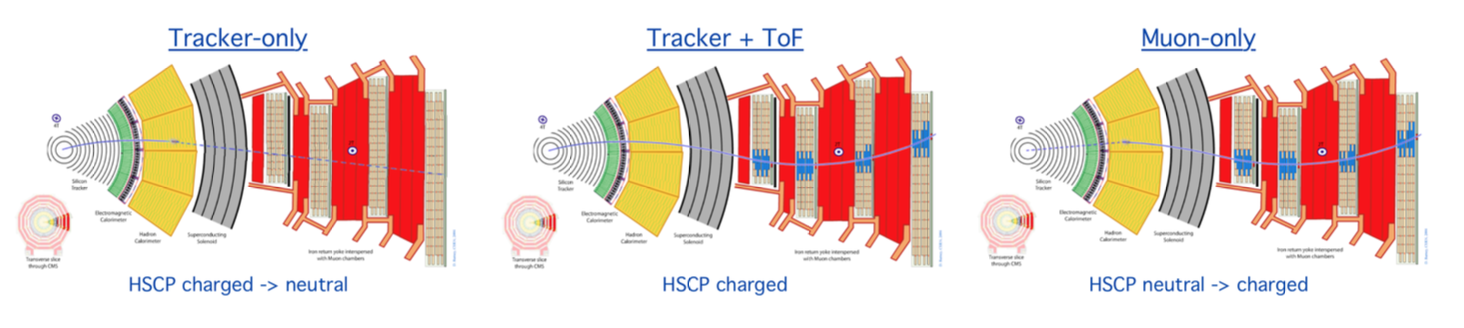
\includegraphics[width=\textwidth]{../ImmaginiTesi/HSCPsearch.png} 
     \caption{Possibili analisi per la ricerca di HSCP: solo sistema di tracking, sistema di tracking e sistema muonico, solo sistema muonico}
   \label{fig:HSCPSearch}
 \end{figure}

In particolare è possibile eseguire tre tipi diverse di analisi in base alla natura dei candidati HSCP, come mostrato in Figura \ref{fig:HSCPSearch} \cite{MasterThesisGioMoc}: 
\begin{itemize}
   \item Analisi solo sul sistema di Tracking adronico, per la ricerca di LLP cariche di tipo adronico che, interagendo con il detector, perdono la carica prima di arrivare al sistema muonico;
   \item Analisi su sistema di Tracking e sistema muonico, per la ricerca di LLP cariche di tipo adronico o muonico;
   \item Analisi solo sul sistema muonico, per la ricerca di particelle neutre che, interagendo con il detector, acquistano carica dopo il sistema di tracking.
\end{itemize}

La rilevazione di queste particelle è però ostacolata dal sistema di Trigger: la collisione di protoni nel punto di origine a CMS avviene con una energia nel centro di massa $\sqrt{s} \approx 14 \si{GeV}$ dunque i prodotti dell'interazione sono particelle con una velocità $\beta \approx 1$ e il Trigger è calibrato per la rilevazione di eventi di questo tipo. Ciò è un problema in quanto, come mostrato in \cite{MasterThesisGioMoc}, l'efficienza di Trigger per particelle con $\beta < 0.6$ decresce molto rapidamente e per tanto la rilevazione di candidati HSCP non è efficiente: la spiegazione è che per velocità ridotte le tracce rilasciate per ionizzazione nel sistema muonico impiegano più di 25ns per attraversare le stazioni di CMS e per tanto il sistema di Trigger muonico riconosce queste tracce come originate da più muoni nel BX corrente e in quello immediatamente successivo.

In questo Capitolo verrà discussa l'implementazione dell'algoritmo utilizzato per la ricerca di eventi compatibili con i modelli di particelle lente. Verranno inoltre mostrati i principali risultati ottenuti, a partire da una analisi a livello delle Stubs del sistema di Data Scouting, spostandosi poi sui corrispondenti candidati muoni emulati del BMTF.

\subsection{Proprietà delle particelle lente}

Tutti i rilevatori DT e RPC della regione di barrel sono sincronizzati per la ricerca di muoni originati nel punto di interazione della collisione dei protoni, ovvero nell'origine del sistema di riferimento di CMS, che si muovono a velocità prossime alla velocità della luce. Un muone da collisione interagisce con i rilevatori, attraversando le quattro stazioni della regione di barrel, in un tempo relativo $t_0 = 0 \si{ns}$ con ampiezza della distribuzione di $t_0$ corrispondente alla risoluzione del tempo di volo \cite{MasterThesisGioMoc}. Particelle lente  potrebbero però attraversare il rilevatore, e quindi le stazioni, in un intervallo temporale maggiore, occupando più bunch crossing, fornendo segnali temporali non compatibili con la calibrazione dei rilevatori DT e RPC. Questi eventi possono essere scartati dal sistema di Trigger, oppure potrebbero essere interpretati come più muoni in BX consecutivi.


\begin{figure}[t]
  \centering
  \centering
  \scalebox{0.75}{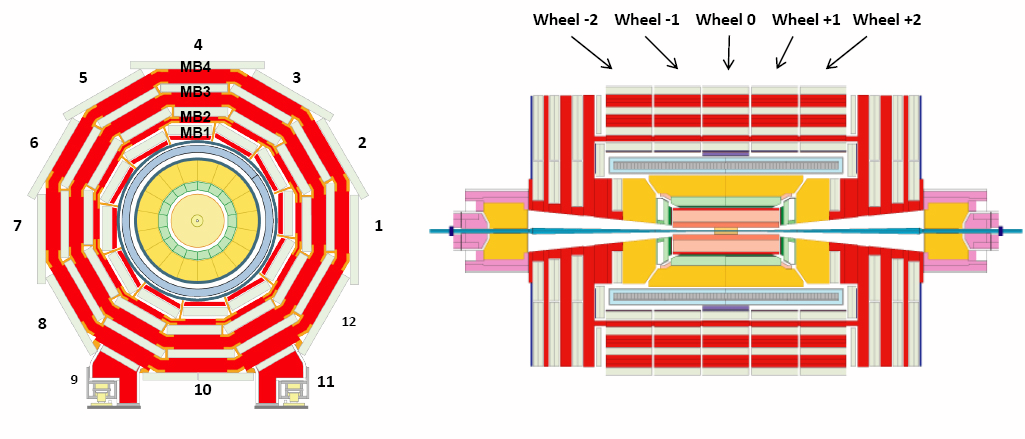
\includegraphics[width=\textwidth]{../ImmaginiTesi/AllCMS.png} }
  \caption{}
  \label{fig:CMSLayout}
\end{figure}


L'algoritmo implementato ricerca le stubs nel bunch crossing successivo (BX+1) che siano \textit{compatibili} con le stubs del bunch crossing corrente (BX). Affinché le stubs possano essere considerate compatibili, devono essere soddisfatte le seguenti condizioni:

\begin{itemize}
  \item La stub nel BX+1 deve essere nella stazione successiva alla stub nel BX;
  \item La stub nel BX+1 deve trovarsi nello stesso sector e wheel della stub nel BX, o in quelli immediatamente adiacenti.
\end{itemize}

%Dalle stubs che rispettano i criteri di compatibilità vengono estratte, nel BX e nel BX + 1, informazioni quali numero di BX, station, sector e wheel di appartenenza.

Come nel Capitolo \ref{cap:SecondoCapitolo} verranno studiati segnali provenienti dalle stubs generate dalle schede TwinMux della regione di barrel per la ricerca di particelle lente.


\begin{figure}[t]
  \centering
  \begin{minipage}[b]{0.48\textwidth}
    \centering
    \includegraphics[width=\textwidth]{../Immagini/NearCompatibleStubs.pdf} 
    \end{minipage}
    \hfill 
    \begin{minipage}[b]{0.48\textwidth}
      \centering
      \includegraphics[width=\textwidth]{../Immagini/PhiCosmicMuons.pdf} 
    \end{minipage}
    \caption{Distribuzione delle stubs compatibili nei settori da 7 a 11 in un sottoinsieme dei possibili bunch crossing (sinistra), distribuzione del numero di stubs compatibili tra BX e BX+1 (destra)}
  \label{fig:MatchedStubsRate}
\end{figure}

\begin{figure}[t]
  \centering
  \begin{minipage}[b]{0.49\textwidth}
    \centering
    \includegraphics[width=\textwidth]{../Immagini/MatchedStubs.pdf} 
    \end{minipage}
    \hfill 
    \begin{minipage}[b]{0.49\textwidth}
      \centering
      \includegraphics[width=\textwidth]{../Immagini/MatchedStubsCombination.pdf} 
    \end{minipage}
    \caption{Distribuzione del numero totale di stubs compatibili tra BX e BX+1 (sinistra), distribuzione delle combinazioni di stubs compatibili tra BX e BX+1 nei casi in cui ci siano 3 o 4 stubs totali}
  \label{fig:MatchedStubsCombination}
\end{figure}

In Figura \ref{fig:MatchedStubsRate} sulla sinistra viene mostrata la distribuzione di stubs nei bunch crossing successivi compatibili con le stubs del BX. La maggior parte degli eventi presenta compatibilità nel BX immediatamente successivo (BX+1), ma vi sono eventi che presentano compatibilità a distanze temporali maggiori: nel seguito della analisi verranno presi in considerazione solamente i primi eventi in quanto è improbabile che particelle lente impieghino più di due BX per attraversare il rilevatore. \newline
In Figura \ref{fig:MatchedStubsRate} sulla destra viene mostrata la distribuzione dei bunch crossing in cui sono state rilevate stubs compatibili nella parte inferiore del rilevatore CMS, ovvero nei settori dal 7 all'11: in questa regione vi sono sia eventi compatibili con fenomeni di collisione, rappresentati dai soliti segnali del filling scheme di LHC, ma anche molti eventi compatibili con segnali derivanti da fondo cosmico. In particolare confrontando Figura \ref{fig:MatchedStubsRate} con Figura \ref{fig:Stubs1} si osserva come il rate di fondo cosmico sia in rapporto maggiore al rate di eventi da collisione: la spiegazione è che i muoni cosmici attraversano costantemente i rilevatori delle camere muoniche e non solo nei BX di collisione e per tanto sono spesso considerati compatibili dall'algoritmo.

In Figura \ref{fig:MatchedStubsCombination} sulla sinistra viene mostrata la distribuzione delle stubs \textit{totali} compatibili tra BX e BX+1: la maggior parte degli eventi presentano compatibilità solamente tra due stubs in bunch crossing differenti, ovvero 1 stub in BX è compatibile con 1 stub nel BX+1. Più interessanti sono però le distribuzioni quando le stubs totali sono tre o quattro: in Figura \ref{fig:MatchedStubsCombination} sulla destra viene mostrato che, quando vi sono tre stubs compatibili, la probabilità che vi siano 2 stubs nel primo BX e 1 in BX+1 è la medesima del viceversa. Quando invece ci sono quattro stubs, la probabilità che 2 stubs ricadano nel primo BX e 2 nel BX+1 è nettamente inferiore rispetto alle altre permutazioni. 



\begin{figure}[t]
  \centering
  \begin{minipage}[b]{0.48\textwidth}
    \centering
    \includegraphics[width=\textwidth]{../Immagini/Pt3And3More.pdf} 
    \end{minipage}
    \hfill 
    \begin{minipage}[b]{0.48\textwidth}
      \centering
      \includegraphics[width=\textwidth]{../Immagini/Qual3And3More.pdf} 
    \end{minipage}
    \caption{Distribuzione del momento trasverso e qualità dei candidati muoni generati da meno di 3 o più di 3 stubs compatibili}
  \label{fig:PtQual3And3More}
\end{figure}




È inoltre interessante ricercare e studiare le proprietà dei muoni del BMTF generati a partire dalle stubs compatibili con le richieste dell'algoritmo, ricordando che questi muoni sono eventi particolari in quanto rappresentano particelle generate da segnali compatibili in bunch crossing adiacenti. 
Di seguito verrà quindi eseguita una analisi più approfondita di questi eventi, in quanto potrebbero rappresentare particelle che impiegano mediamente più tempo per attraversare le stazioni del rilevatore, ovvero potrebbero essere considerate \textit{lente}.\newline
Quindi, a partire dalle informazioni sulle stubs, è possibile ricondursi ai muoni generati dal Barrel Muons Track Finder: come esposto nel Capitolo \ref{cap:SecondoCapitolo} infatti, il sistema di tracking della regione di barrel ricostruisce i muoni a partire da almeno due stubs generate dalle schede TwinMux, fornendo informazioni circa il momento trasverso del muone, la qualità, oltre che informazioni spaziali come $\phi$ ed $\eta$. 

Vengono inizialmente studiati i muoni generati da 3 e da 4 stubs, verificandone le differenze. Verifichiamo prima di tutto che il numero totale di muoni nei due casi è molto diverso: vi sono ... muoni generati da 3 stubs e ... da 4 stubs su un totale di 5.22 minuti di presa dati. In Figura \ref{fig:PtQual3And3More} sulla sinistra viene mostrata la distribuzione del momento trasverso di questi muoni: si nota che non vi è una particolare differenza tra le due distribuzioni a basso momento mentre, probabilmente a causa della bassa statistica di eventi di questo tipo, la distribuzione ad elevato momento risolta poco popolata in entrambi i casi. Sulla destra di Figura \ref{fig:PtQual3And3More} invece è rappresentata la qualità associata ai muoni generati dalle stubs: il sistema di Tracking assegna la qualità ad un muone in base al numero di stubs da cui è formato, pertanto come ci si aspetta, muoni formati da 3 stubs hanno generalmente una qualità inferiore a quelli formati da 4 stubs.

\begin{figure}[t]
  \centering
  \begin{minipage}[b]{0.48\textwidth}
    \centering
    \includegraphics[width=\textwidth]{../Immagini/BXDiff.pdf} 
    \end{minipage}
    \hfill 
    \begin{minipage}[b]{0.48\textwidth}
      \centering
      \includegraphics[width=\textwidth]{../Immagini/DeltaPt.pdf} 
    \end{minipage}
    \caption{Differenza tra BX dei muoni formati da 2 stubs in BX e BX+1 e BX da collisione (sinistra), distribuzione della differenza del momento tra i due muoni in BX e BX+1 (destra)  }
  \label{fig:BXDiffAndPt}
\end{figure}

\begin{figure}[t]
  \centering
  \begin{minipage}[b]{0.48\textwidth}
    \centering
    \includegraphics[width=\textwidth]{../Immagini/DeltaPhi.pdf} 
    \end{minipage}
    \hfill 
    \begin{minipage}[b]{0.48\textwidth}
      \centering
      \includegraphics[width=\textwidth]{../Immagini/DeltaEta.pdf} 
    \end{minipage}
    \caption{ distribuzione della differenza dell'angolo $\phi$ tra i due muoni in BX e BX+1 (sinistra), distribuzione della differenza $\eta$ tra i due muoni in BX e BX+1 (destra)}
  \label{fig:DeltaETaDeltaPhi}
\end{figure}

Dalla Figura \ref{fig:MatchedStubsCombination} si nota come solamente una minoranza degli eventi presenti due stubs nel BX compatibili con due stubs nel BX+1. Sapendo che dal sistema di Tracking sono necessarie almeno due stubs per generare un candidato muone, è possibile ricercare tra questi eventi quelli che presentano un muone nel BX e uno nel BX+1, generati dalle stubs di cui prima. \newline
Queste coppie di muoni sono eventi particolari: sono muoni in BX adiacenti generati da due stubs ognuno, le quali sono \textit{compatibili}, ovvero per la definizione di compatibilità fornita ad inizio della sezione, stubs che percorrono tutte e quattro le stazioni della regione di barrel, rimanendo sempre negli stessi sector e wheel, o in quelli adiacenti. In genere ci si aspetta che non siano presenti eventi di questo tipo, in quanto rappresenterebbero evidentemente lo stesso muone, percepiti però dal sistema di Trigger come due muoni in due BX separati.

In realtà si scopre che in 5 minuti e 22 secondi di presa dati sono presenti all'incirca 200 eventi di questo genere. Come prima cosa è possibile verificare che questi eventi siano generati dalla collisione di protoni e che non siano quindi associabili ad un fondo cosmico: per farlo è possibile studiare in che bunch crossing questi eventi sono stati rilevati, confrontandolo con il filling scheme mostrato in Figura \ref{fig:BMTFMuons}. In Figura \ref{fig:BXDiffAndPt} sulla sinistra viene mostrata la distribuzione della differenza tra i BX degli eventi in esame con i BX di collisione: la maggior parte degli eventi ricadono proprio nei BX da collisione, o in quelli immediatamente adiacenti, siamo dunque portati ad affermare che gli eventi in esame siano tutti derivanti da fenomeni di collisione. In caso contrario infatti ci aspetteremmo che la distribuzione fosse popolata in modo più omogeneo anche nei BX dove non sono presenti interazioni tra protoni.

È possibile quindi studiare la distribuzione della differenza di momento e di posizione spaziale tra questi eventi per verificare che le due particelle nei due BX adiacenti siano \textit{simili}, ovvero che possano rappresentare la stessa particella. In Figura \ref{fig:BXDiffAndPt} sulla destra e in Figura \ref{fig:DeltaETaDeltaPhi} viene mostrata la differenza di momento trasverso $p_T$, pseudorapidità $\eta$ e  angolo $\phi$: tutte queste distribuzioni sono centrate sullo zero.



%----------------POSSIBILE CONCLUSIONE----------------

Nonostante questi segnali siano promettenti e provino la possibile esistenza di particelle lente generate dalla collisione di protoni ad elevata energia, le informazioni a disposizione non sono complete: il tempo di volo delle particelle è un discriminante fondamentale per il riconoscimento di particelle che si muovono a velocità molto minori della velocità della luce. Sia i rilevatori Drift Tubes che i Cathode Strip Chambers permettono misurazioni temporali precise, ma sono calibrate per la ricerca di particelle in moto ultrarelativistico: per HSCP lente i segnali derivanti dai DT sarebbero ricostruiti in modo non accurato a causa della velocità non compatibile con quella della luce, generando un pattern a zigzag nella ricostruzione temporale traslato di un offset proporzionale al ritardo $\delta_t$ del segnale nel DT. Conoscendo il ritardo si determina la velocità della particella \cite{CMS-PAS-EXO-16-036}:

\begin{equation}
  \label{eq:Velocity}
  \beta^{-1} = 1 + \frac{c\delta_t}{L}
\end{equation}

Dove $L$ è la distanza percorsa nel tempo di volo, definita in Equazione \ref{eq:LorentzBoost}.

